\documentclass[a4paper,11pt]{report}
\usepackage[T1]{fontenc}
\usepackage[utf8]{inputenc}
\usepackage{lmodern}
\usepackage[francais]{babel}
\usepackage[top=2cm,left=2.2cm,right=2.2cm,bottom=2cm]{geometry} % Géométrie de la page, modifier selon le besoin
\usepackage{lmodern, wrapfig, textcomp, tikz, graphicx, amsmath, tikz-qtree, xcolor,rotating,epic,eepic}
\usepackage[colorlinks,linkcolor=black, urlcolor=blue]{hyperref}
\usepackage[babel=true,kerning=true]{microtype}
\usepackage{url}
\usepackage{caption}
\usepackage{subcaption}
\usepackage{array}% http://ctan.org/pkg/array
\date{}
\title{}
\author{}

\begin{document}
\nocite{*}
\pagenumbering{gobble}  % Pas de numérotation
\begin{titlepage}
        \vspace*{1cm}

\includegraphics[scale=0.45]{Images/logo_phelma.pdf}
    \begin{flushright}
        %\vspace*{-3cm}
        %\includegraphics[scale=0.3]{Images/}
        %\vspace*{-2cm}
    \end{flushright}
\begin{center}
    \vspace*{2cm}
    \rule{\linewidth}{0.5mm}\\[0.4cm]
    {\huge\bfseries Projet de Recherche\\
    [0.4cm]}\rule{\linewidth}{0.5mm}\\[0.5cm]
    \large{\textsc{Léo Friedrich, Paul Noël, Luca Panat, Félix Piédallu}}\\[2cm]
    \large{\textsc{Tuteur : Frank Balestro}}\\[2cm]

%\includegraphics[scale=0.64]{Images/LogoPNS}

\end{center}
\end{titlepage}

\tableofcontents        % Table des matières avec liens, générée automatiquement.
\newpage
\pagenumbering{arabic}  % Numérotation de retour !


\begin{abstract}
L'équipe avec laquelle s'est effectué notre projet de recherche est l'équipe Nanospintronique et Transport Moléculaire de l'institut Louis Néel. Et c'est en particulier Franck Balestro qui nous a encadré lors de l'expérience et en amont de celle-ci.\\
\begin{figure}[h]
    \begin{center}
        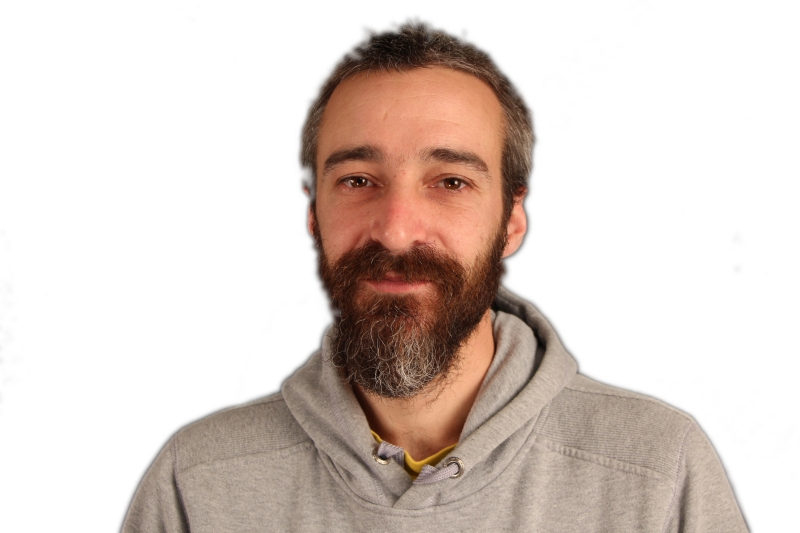
\includegraphics[height=133px]{Images/Balestro-trim.jpg}
        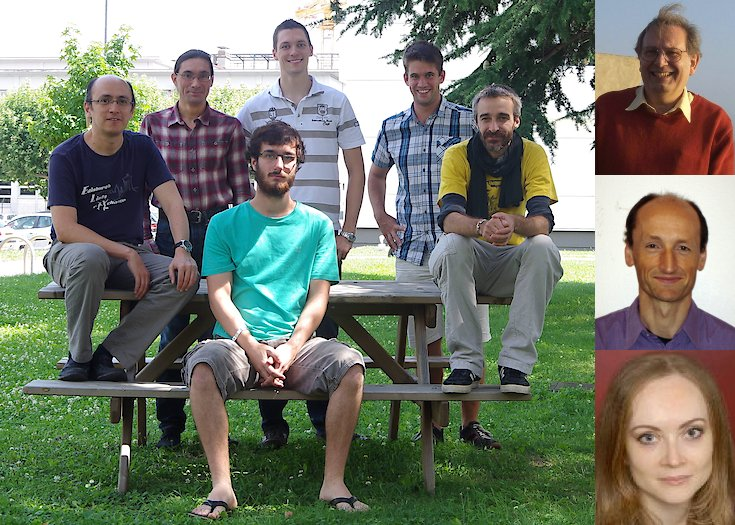
\includegraphics[height=133px]{Images/NanoSpin.jpg}
        \caption{Frank Balestro et l'équipe NanoSpin}
        \label{fig:}
    \end{center}
\end{figure}
                                             
L'équipe travaille à la manipulation et à la lecture de spins nucléaires uniques, c'est à dire relier le monde quantique au monde macroscopique et permettre à terme l'avènement de l'informatique quantique. Pour ce faire ils utilisent des molécules ayant des propriétés spécifiques: les aimants moléculaires, d'excellents candidats pour le stockage et le traitement de l'information quantique.\cite{1} Les molécules étant de plus de très petite taille comparativement aux dimensions des transistors utilisés en électronique classique, elles pourraient permettre d'améliorer la densité des circuits. Pour résumer et comme le dit Franck Balestro l'objectif de l'équipe est "de créer l'électronique du futur avec des molécules"\cite{2}.\\

Les enjeux sont donc immenses, particulièrement dans un contexte où la réduction des dimensions des transistors devient de plus en plus problématique et où le besoin en puissance de calcul de nos ordinateurs devient de plus en plus important ; une "nouvelle électronique" peut être la solution.\\

Pour notre part nous avons réalisé un transistor à molécule unique à l'aide de fullerène. Une telle molécule ne possède pas de propriété particulière mais permet de comprendre le fonctionnement général des transistors à molécule unique. Historiquement, c'est la toute première molécule utilisée pour ce type de réalisation en 2000 par l'équipe de Park\cite{13}.
\end{abstract}

\chapter{État de l'art}
\section{L'idée d'une électronique moléculaire}
C'est en 1974 que l'idée d'utiliser des molécules uniques dans la fabrication de composants électroniques est apparue, lors d'un séminaire tenu par Arieh Aviram et Mark Ratner.

Cette date peut être considérée comme la naissance de ce que l'on appelle l'électronique moléculaire.
Le but étant à la fois de permettre d'aller encore plus loin dans la miniaturisation des composants en microélectronique mais aussi d'adopter une technique de fabrication basée sur l'auto-organisation de petites molécules en structure complexe: technique dite “bottom-up”.
\section{Le premier transistor moléculaire}
Mais en 1974, on est encore loin de l'utilisation concrète de molécules uniques dans l'électronique, et il faudra attendre 1995 pour que la première mesure de courant à travers une molécule unique soit réalisée à l'aide d'un microscope à effet tunnel (STM).

De nombreuses autres expériences vont suivre, et en 1997 apparaît la technique de “break junction” qui consiste à effectuer la cassure d'un pont métallique sur substrat flexible en pliant le substrat. On peut alors sans STM mesurer les caractéristiques de molécules uniques, et caractériser l'influence de la taille du gap. Mais on n'a toujours pas de grille pour pouvoir permettre l'utilisation comme transistor.

Ce n'est qu'en 2000 que J.W. Park et son équipe utiliseront une technique d'électromigration\footnote{Nous présentons plus en détail l'électromigration dans une partie dédiée.} pour permettre la fabrication du premier transistor à molécule unique avec une molécule de fullerène C$_{60}$. D'autres groupes vont alors utiliser cette même technique en utilisant d'autres molécules et leurs propriétés, et en particulier des aimants moléculaires (SMM) pour leurs propriétés liées au spin. Mais aussi en mettant en place des expériences qui permettront d'effectuer les mesures à quelques milliKelvins.

\section{De nouvelles molécules: vers la spintronique moléculaire}
En 2006 l'utilisation de SMM débute afin de permettre la réalisation de dispositifs de spintronique moléculaire. Les équipe de H.S.J Van der Sant (à Cornell) et D.C. Ralph (à Delft) vont étudier tout d'abord l'aimant moléculaire le plus fameux, Mn$_{12}$, mais les résultats sont peu satisfaisants et la première réalisation d'un véritable dispositif de spintronique moléculaire est réalisé à Delft par l'équipe de Ralph en 2008 à l'aide d'une molécule de N@C$_{60}$ (atome d'azote piégé dans une molécule de fullerène). Il est possible avec une telle molécule de retrouver dans les mesures de transport ses propriétés magnétiques.\\

\begin{figure}[h]
    \begin{center}
        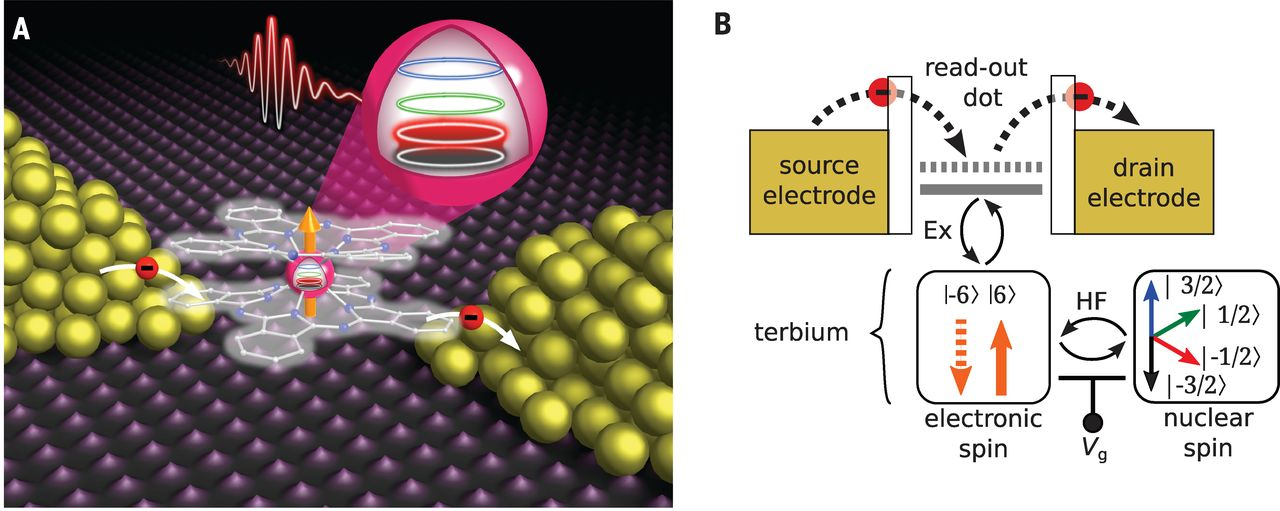
\includegraphics{Images/TbPc2.jpg}
        \caption{Vue de la molécule de TbPc$_2$, et schéma de principe.}
        \label{fig:}
    \end{center}
\end{figure}

Cependant cette molécule n'est pas un aimant moléculaire, et il impossible donc de se servir des propriétés quantiques liées au magnétisme moléculaire. Les équipes vont donc se tourner vers d'autres aimants moléculaires notamment Fe$_{4}$ (à Delft), Ni$_{4}$(à Cornell)...etc et la molécule TbPc$_{2}$ (molécule organique avec un atome de Terbium) à l'institut Louis Néel dans l'équipe de Franck Balestro. L'aimant moléculaire TbPc$_{2}$ utilisée dans un transistor à molécule unique a permis de réaliser la lecture électrique et la manipulation quantique d'un spin nucléaire unique.

\chapter{Aspects théoriques}
\section{Le testeur sous pointes et ADWin}
Pour réaliser l'électromigration, on a besoin du testeur sous pointes qui, grâce à ses quatre bras orientables supportant les pointes, permet d'imposer une rampe de tension et de mesurer simultanément la conductance. Le testeur sous pointe possède un accès optique permettant de connecter rapidement les échantillons et de les refroidir à 4,2K. Notons que le contact est moins bon qu'avec des microsoudures.

\begin{figure}[h]
    \begin{center}
        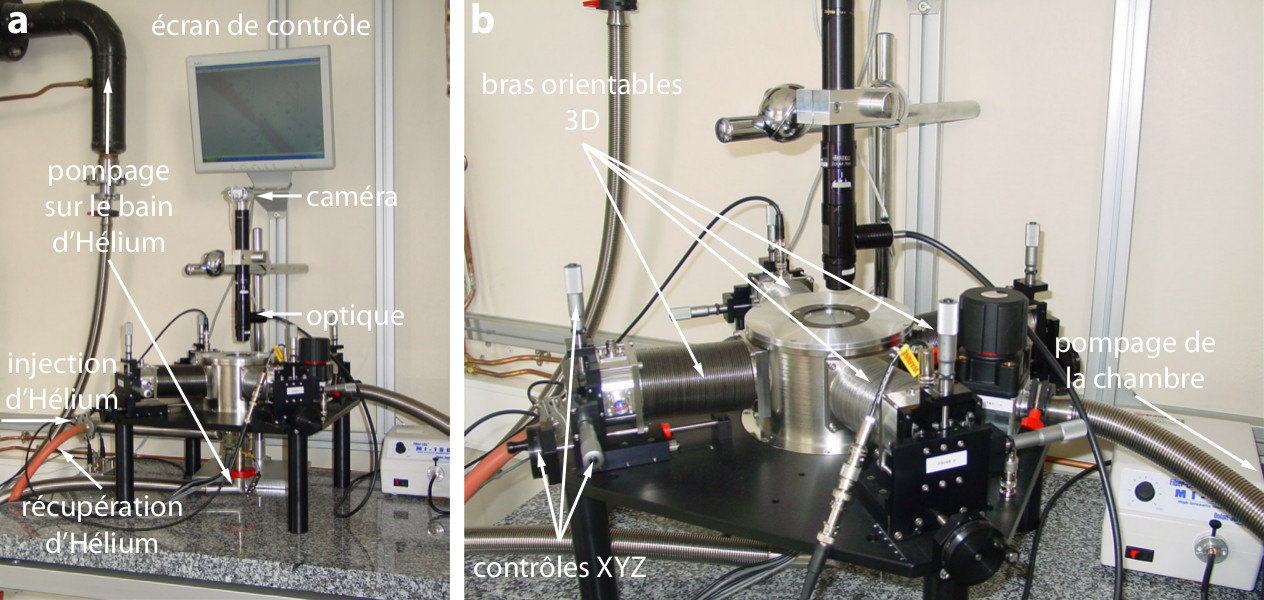
\includegraphics[width=250px]{Images/2_ADWin_avec_legendes}
        \caption{Le Testeur sous Pointes}
        %Photo disponible à \url{https://tel.archives-ouvertes.fr/tel-00456601v2/document}
    \end{center}
\end{figure}
On doit disposer d'une électronique de mesure en temps réel et d'une détection synchrone : c'est le rôle d'ADWin.

La première partie constituant ADWin est l'ordinateur permettant le stockage des données et l'interface graphique. Vient ensuite le processeur propre à ADWin qui garantit la répétition de suites d'instructions toutes les 3,3ns. Ceci est une nécessité car un OS (multitâche) ne pourrait garantir une base de temps inférieure à 10ms et compromettrait le résultat de l'électromigration. Enfin les convertisseurs génèrent et reçoivent les signaux expérimentaux.

\begin{figure}[h]
    \begin{center}
        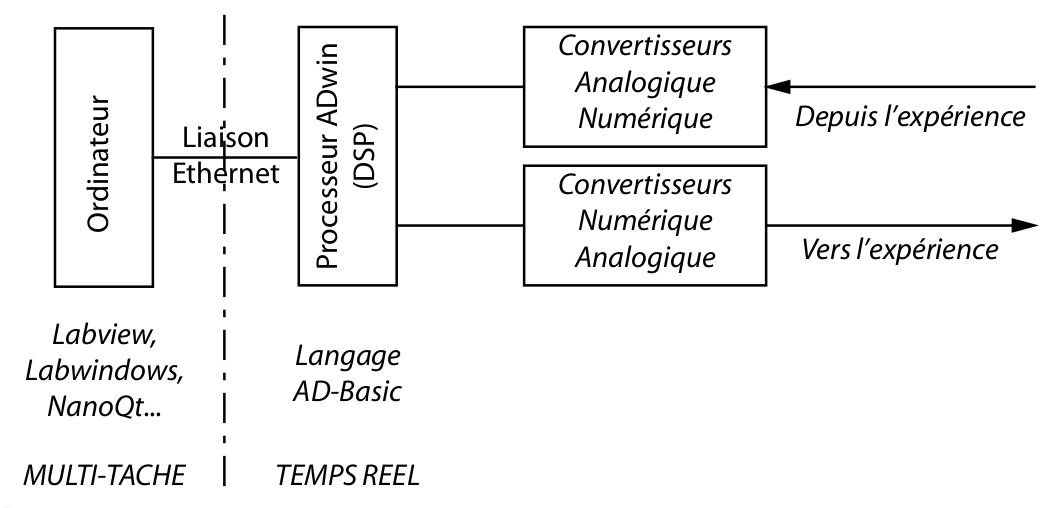
\includegraphics[width=250px]{Images/2_ADWin_schema}
        \caption{Schéma de fonctionnement d'ADWin}
        %Schéma disponible à \url{https://tel.archives-ouvertes.fr/tel-00456601v2/document}
    \end{center}
\end{figure}

Un des autres avantages d'ADWin est la diminution du bruit. En incrémentant bit par bit des rampes de mesures (tension, courant) et grâce à la très petite base de temps du système on peut balayer des plages entières de tension, courant, charges en des temps très faible et obtenir une très bonne précision.

\section{Le fullerène}
Les fullerènes sont des molécules composées de carbone d'un nanomètre de diamètre. Leur découverte en 1985 a donné lieu au prix Nobel de chimie 1996 et à toute une nouvelle classe de matériau massique. Le fullerène utilisé est le C$_{60}$, une molécule très simple de la forme d'un ballon de football.

\begin{figure}[h]
    \begin{center}
        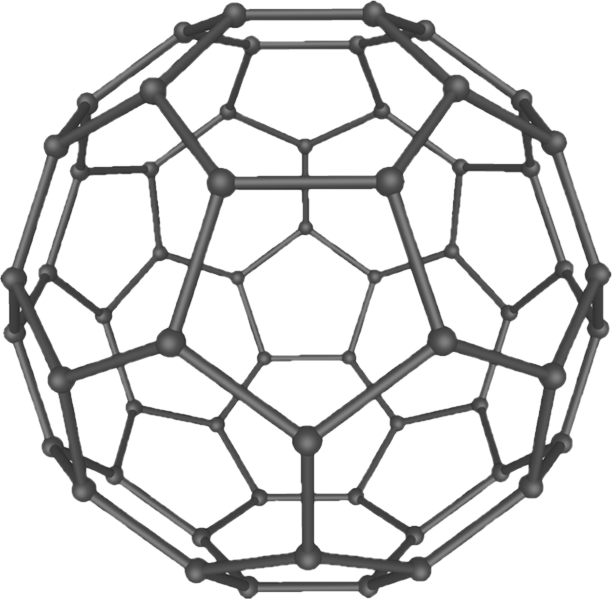
\includegraphics[width=100px]{Images/2_C60.png}
        \caption{Structure de la molécule de Fullerène}
    \end{center}
\end{figure}

On dépose le fullerène C$_{60}$ avant l'étape d'électromigration et on espère qu'une molécule tombe dans le gap créé sur le nanofil d'or. La probabilité d'occurrence est plus importante que si l'on essaye de déposer une molécule dans un gap préexistant. On essaye d'avoir des molécules uniques de C$_{60}$ plutôt que des agrégats car la molécule unique présente une énergie de charge plus importante et un couplage à l'environnement moins fort gage de stabilité. Une dilution dans le toluène permet de caractériser si une solution est composée de molécules uniques (couleur jaune) ou d'agrégats (couleur violette).


\section{L'électromigration}
L'électromigration est un phénomène bien connu en microélectronique. Il s'agit d'un transport de matière observé dans les métaux traversés par de fortes densités de courant ; c'est une cause d'endommagement des interconnexions métalliques et donc de fiabilité dans les circuits intégrés\cite{8}. Ce phénomène est néfaste pour la microélectronique "classique", mais son utilisation est très intéressante pour la réalisation de transistors à molécule unique. En effet il faut que la molécule soit reliée à un dispositif métallique macroscopique et donc que les électrodes (source-drain) soient séparées d'une distance nanométrique proche de la taille de la molécule ; ce qui est impossible par des méthodes de nanofabrication limitées à environ 10nm de résolution, alors qu'une résolution inférieure est possible grâce à l'électromigration\cite{9}.\medskip 

Intéressons-nous maintenant à la description théorique de l'électromigration, "mise en mouvement des atomes par un métal causée par l'application d'un champ électrique". La force de transport peut être notée :
\[\vec{F}=e Z^* \vec{E}\]
où le terme $Z^*$ se décompose en deux parties, l'une modélisant l'effet du champ électrostatique, l'autre le "vent des électrons" qui transmettent leurs mouvements aux ions.
\[Z^* = Z_{\text{electrostatique}} + Z_{\text{vent}}\]
Dans les métaux c'est principalement le vent d'électrons qui est responsable du transport, ainsi le transport de matière a lieu dans le sens de circulation des électrons\cite{10}.\medskip 

Il faut maintenant pouvoir suivre l'électromigration pour pouvoir réaliser un nanogap, cela est possible grâce à une mesure en temps réel de la conductance (ou la résistance) à l'aide d'ADWin.\medskip 

Au cours de l'électromigration, les propriétés de conduction vont évoluer et on peut distinguer deux régimes de conduction :
\begin{description}
    \item[Le régime diffusif,] lorsque le libre parcours moyen ($L_m \simeq 10nm$) est inférieur aux dimensions du nanofil
    \item[Le régime ballistique,] lorsque le libre parcours moyen est supérieur aux dimensions du nanofil
\end{description}

Or dans le cas du régime balistique, d'après la formule de Landauer Buttiker, la conductance est un multiple du quantum de conductance :
\[G = G_0 \sum_{n=1}^N T_n \quad \text{ où } \quad G_0 = \frac{2e^2}{h} = 77.5 \mu S\]
avec les T probabilités de transmission pour les N canaux de conduction.
\begin{figure}[h]
    \begin{center}
        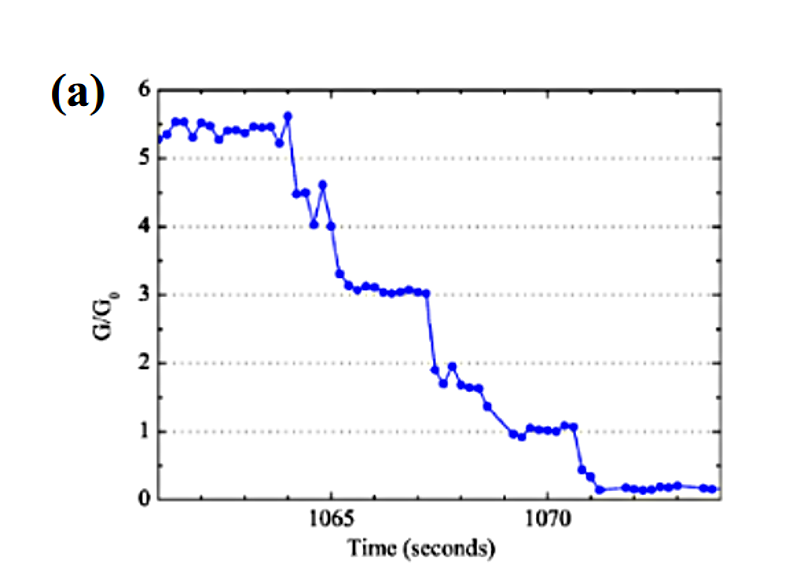
\includegraphics[width=250px]{Images/2_Electromigration_graphe}
        \caption{Variation de G en fonction du temps à la fin d'une électromigration (au moment de l'ouverture du nanogap).
On observe bien des paliers de conductance.}
        %Photo disponible à \url{https://tel.archives-ouvertes.fr/tel-00515127/document}
    \end{center}
\end{figure}

On en déduit ainsi que si G<G${_0}$ ou R>R${_0}$, il n'y a plus de canaux de conduction et donc qu'on a crée un nanogap. Il suffit donc de stopper l'électromigration à cette limite de conductance dans un temps très court de l'ordre de la microseconde ce qui est possible grâce à l'électronique temps réel\cite{11}.

En réalité on stoppera plutôt notre expérience à R>2R${_0}$ qui expérimentalement assure de meilleurs résultats.

\section{Le blocage de Coulomb dans un transistor à électron unique}
\footnote{Cette partie s'inspire librement du cours de nanophysique de Monsieur Thierry Ouisse de 2A PNS ainsi que des aspects théoriques présentés dans \cite{3}, \cite{5}, \cite{10}, \cite{13} et \cite{15} qui présentent en détail le blocage de Coulomb.}
On considère un îlot quantique, placé entre 3 électrodes : le drain, la source et la grille. Le drain et la source sont séparés de l'îlot par des jonctions tunnels. On note V${_d}$, V${_s}$ et V${_g}$ respectivement les tensions de drain, source et grille. De plus, on note N le nombre d'électrons à l'intérieur de l'îlot. 
\begin{figure}[h]
    \begin{center}
        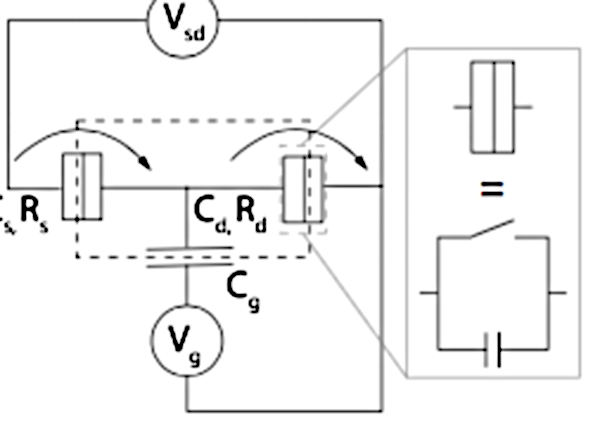
\includegraphics[width=250px]{Images/2_Blocage_Coulomb_Schema}
        \caption{Schéma équivalent du transistor}
    \end{center}
\end{figure}

L'îlot possède donc une énergie électrostatique E${_c}$.

Ainsi, il va falloir apporter de l'énergie à un électron pour pouvoir le faire rentrer dans l'îlot Quantique. Si $V_{sd}>0$, il va être plus simple  d'injecter un électron dans l'îlot depuis la source plutôt que depuis le drain. Une fois l'électron apporté dans l'îlot, on modifie l'énergie à l'intérieur de l'îlot, ce qui va rendre plus difficile l'entrée d'un nouvel électron (on passe de N à N+1). Cette variation d'énergie doit être négative si l'on veut continuer à faire rentrer des électrons:
\[\Delta E = \frac{e}{C_1 + C_2 + C_G}\left((N + \frac{1}{2})e - C_G V_G - C_2 V_D\right)\]
ce qui donne la condition :
\[V_D > (N + \frac{1}{2})\frac{e}{C_2} - \frac{C_G}{C_2}V_G\]

De manière analogue, si $V_{sd}>0$, il va être plus facile de sortir un électron de l'îlot par le drain que par la source (on passe de N à N-1). On va cette fois ci avoir une variation d'énergie positive si l'on veut arrêter de faire rentrer des électrons dans l'îlot :
\[\Delta E = \frac{e}{C_1 + C_2 + C_G}\left(-(N + \frac{1}{2})e + C_G V_G - (C_1 + C_G) V_D\right)\]
(car il va être plus simple de rentrer un nouvel électron). Cette variation va donner la condition:
\[V_D > - (N + \frac{1}{2})\frac{e}{C_1 + C_G} + \frac{C_G}{C_1 + C_G}V_G\]

De même, en refaisant le raisonnement pour $V_{sd}<0$. Dans ce cas, il sera plus simple de rentrer un électron dans l'îlot à partir du drain et d'en sortir un à partir de la source. On obtient deux nouvelles conditions similaires au cas où  $V_{d}>0$ :
\[V_D < - (N + \frac{1}{2})\frac{e}{C_1 + C_G} + \frac{C_G}{C_1 + C_G}V_G\]

\[V_D < (N + \frac{1}{2})\frac{e}{C_2} - \frac{C_G}{C_2}V_G\]

À présent, on peut visualiser les diamants de Coulomb et les domaines de blocage de Coulomb quand on trace les droites dans le plan ($V_{sd}$,$V_{g}$). Quand on est sur une droite, on a dans l'îlot N électrons. Ces droites coupent l'espace ($V_{sd}$,$V_{g}$) en 2 demi-plans avec chacun une certaine condition (impossibilité de faire transiter un électron par la source ou le drain par exemple).
\begin{figure}[h]
    \begin{center}
        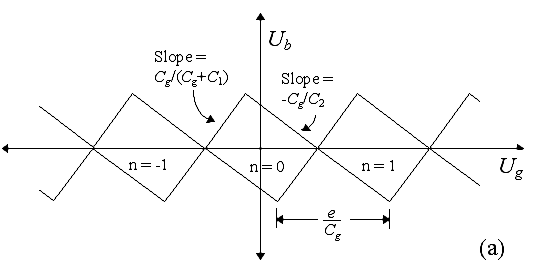
\includegraphics[width=250px]{Images/2_Diamant_Coulomb_Theorie.png}
        \caption{Diamant de Coulomb théorique}
    \end{center}
\end{figure}

Quand on est à l'intérieur d'un de ces diamants, nous ne pouvons plus faire circuler d'électrons dans l'îlot. Quand nous sommes au-dessus ou en dessous d'un de ces diamants, il y a possibilité de faire rentrer puis sortir un électron un par un.

Il y a ainsi des pics de conductance pour certaines valeurs de tension de grille lorsque la dégénérescence entre les états de charges N et N+1 est atteinte. On appelle ces pics, pics de Coulomb.

Notre molécule unique de fullerène peut effectivement être considérée comme un point quantique, de par sa géométrie et sa taille. En effet elle est d'une taille de l'ordre d'un nanomètre, taille comparable à la longueur d'onde de Fermi ; il est donc raisonnable de penser que les électrons sont localisés dans les trois dimensions de l'espace.


\chapter{Réalisation de l'expérience}
L'expérience que nous avons réalisé consiste donc à réaliser des transistors moléculaires, afin de caractériser leur comportement.
\section{La réalisation des circuits en salle blanche (faite en amont par Mr Balestro)}
La réalisation des fils d'or a pris plusieurs semaines ; c'est pourquoi Frank Balestro les avait déjà réalisés en salle blanche, au CNRS, avant l'expérience.
Nous avons donc commencé la journée avec 3 plaques de Al$_2$O$_3$, avec chacune 4 groupes de 12 transistors non formés.
\begin{figure}[h]
    \begin{center}
        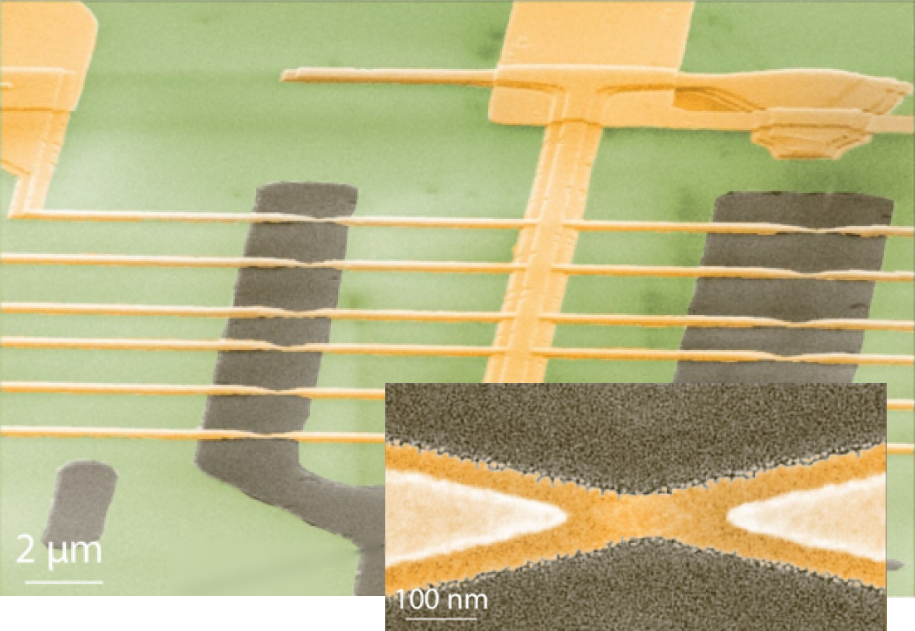
\includegraphics[width=250px]{Images/GroupeDeTransistors}
        \caption{Un groupe de transistors avec grille et source communes}
        \label{fig:}
    \end{center}
\end{figure}
\section{Le dépôt de Fullerène}
Nous sommes donc allés en salle propre de dépôt chimique afin de déposer sur ces plaques le Fullerène, en solution de Toluène.
Cette solution, conservée dans un frigo, est parfaitement inerte, ce qui nous autorise à la conserver très longtemps : celle que nous avons utilisé date de 2009 et est encore utilisable.\\

Le dépôt se fait à l'aide d'une micropipette, et sous hotte aspirante afin d'éviter toute inhalation de fullerène et toute pollution de l'échantillon.
La solution est assez faible en agrégats, et ceux qui ont pu se former se trouvent essentiellement à la surface et au fond de la solution. Nous sommes donc allés récupérer la solution au milieu du bécher.

Le dépôt de fullerène n'a pas besoin d'être mesuré : 3 gouttes de solution par plaque sont suffisantes pour obtenir une probabilité acceptable qu'une molécule se glisse dans le nanogap après électromigration.

Enfin, nous avons laissé s'évaporer le Toluène naturellement.
\section{Une expérience à 4.2K grâce à l'hélium liquide}
Une fois le Fullerène déposé, nous avons fixé les plaques sur un plateau. La fixation se fait à la laque d'argent.

Dans le testeur sous pointes, l'échantillon sera dans une cavité sous vide (vide secondaire de l'ordre de 4-10 millibars). L'unique contact thermique avec les échantillons sera donc par ce plateau. Celui-ci doit être efficace. Sinon, les échantillons seront à haute température et nous n'aurons donc pas du tout le comportement attendu.

L'argent est un très bon conducteur thermique et la laque d'argent permet d'avoir un contact uniforme entre les échantillons et le plateau.

De plus, l'argent nous permet d'avoir une bonne mise à la masse des échantillons et donc de minimiser les risques de choc électrique qui risqueraient de détruire les jonctions formées.
\begin{figure}[h]
    \begin{center}
        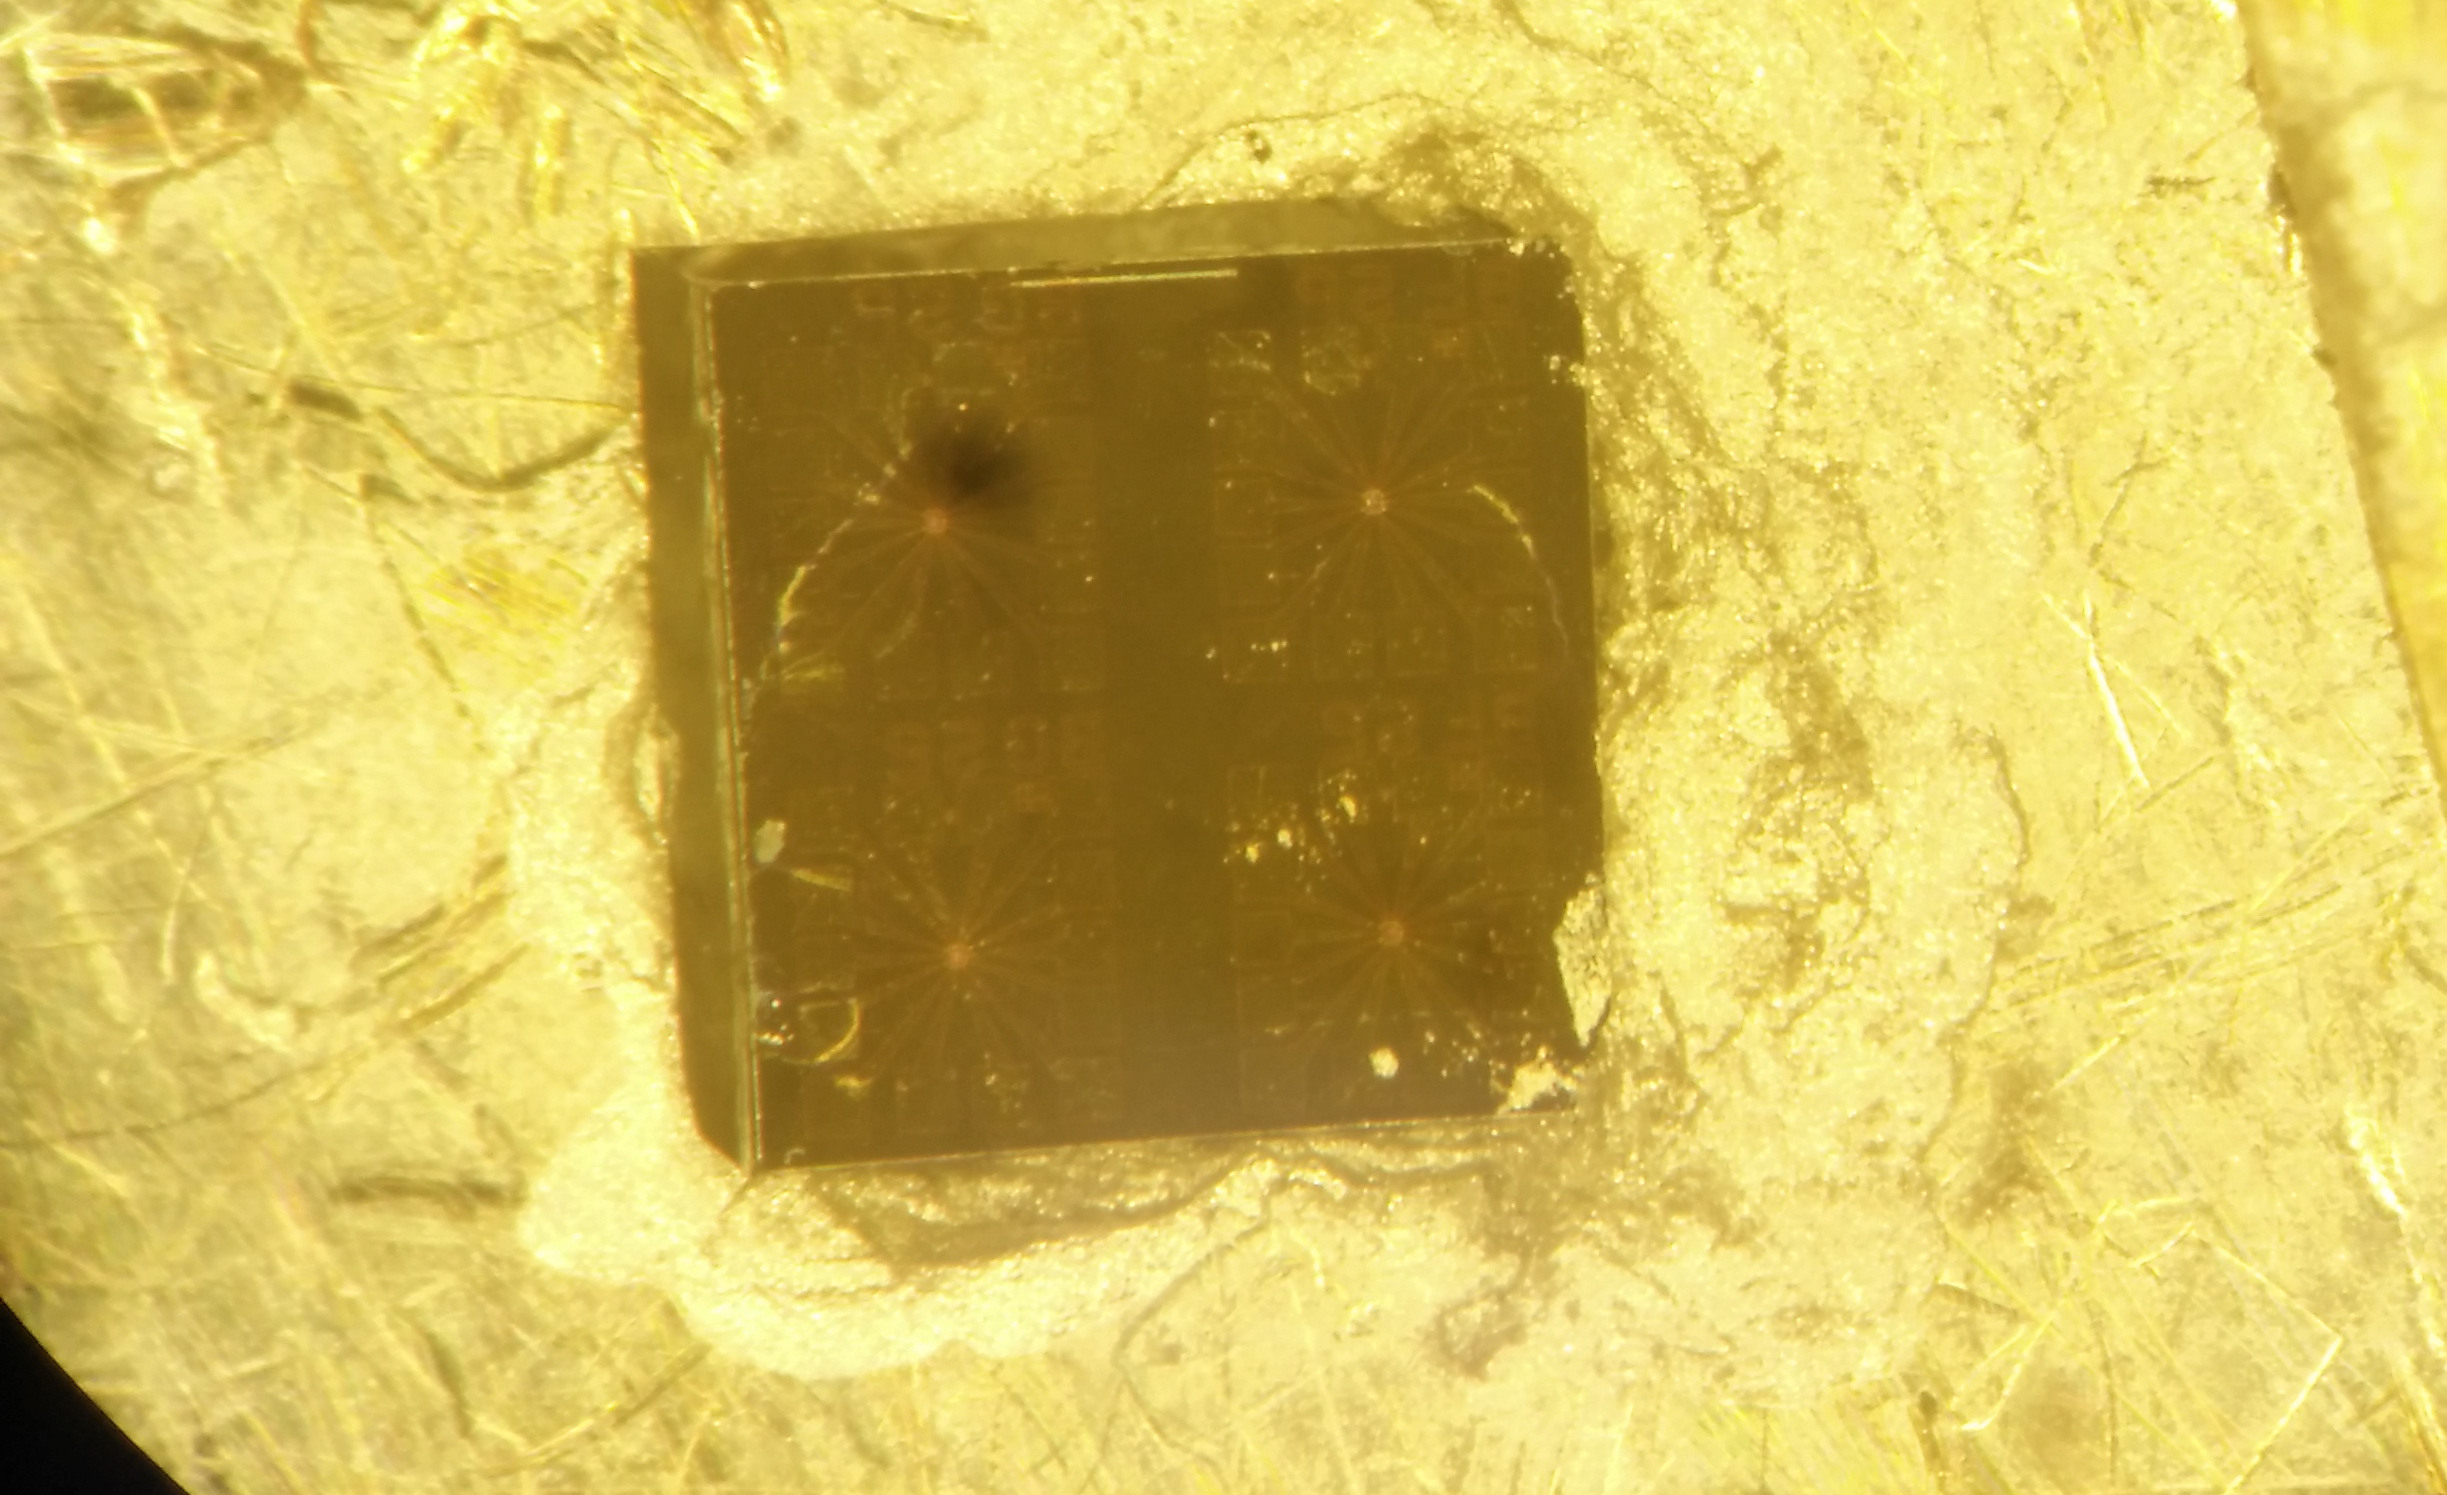
\includegraphics[width=250px]{Images/PhotoPlaqueTransistors}
        \caption{Échantillon collé à l'aide de laque d'argent}
        \label{fig:}
    \end{center}
\end{figure}

Pour empêcher un maximum le réchauffement du au rayonnement l'échantillon est placé sous deux écrans. Le premier  écran est à 10K est placé au niveau du hublot. Le deuxième écran est à 300K (température de la pièce). On peut alors efficacement refroidir à 4.2K. Au préalable, il a fallu faire le vide entre les deux écrans et l'écran intermédiaire et l'échantillon pour empêcher tout réchauffement par conduction ou convection et  pour empêcher que l'air ne gèle autour de l'échantillon ce qui interdirait toute manipulation.
\subsection{L'Hélium Liquide}
Comme dit précédemment, nous pouvons effectuer cette expérience à 4.2K grâce à l'Hélium liquide. Et, heureusement, l'hélium liquide est facile d'accès à l'Institut Néel.

Il nous faut donc transporter la bouteille d'hélium liquide vide jusqu'au centre de liquéfaction, pour prendre une bouteille pleine. Il faut aussi indiquer les poids des bouteilles entrante et sortante, afin d'attribuer la consommation à tel ou tel laboratoire.

La manipulation de la bouteille d'hélium doit se faire avec précaution. En effet, le haut de la bouteille est “chaud”, donc en cas de contact brusque avec l'hélium liquide, celui-ci se dilate très rapidement, ce qui transforme la bouteille d'hélium en “torpille”.
\begin{figure}[h]
    \begin{center}
        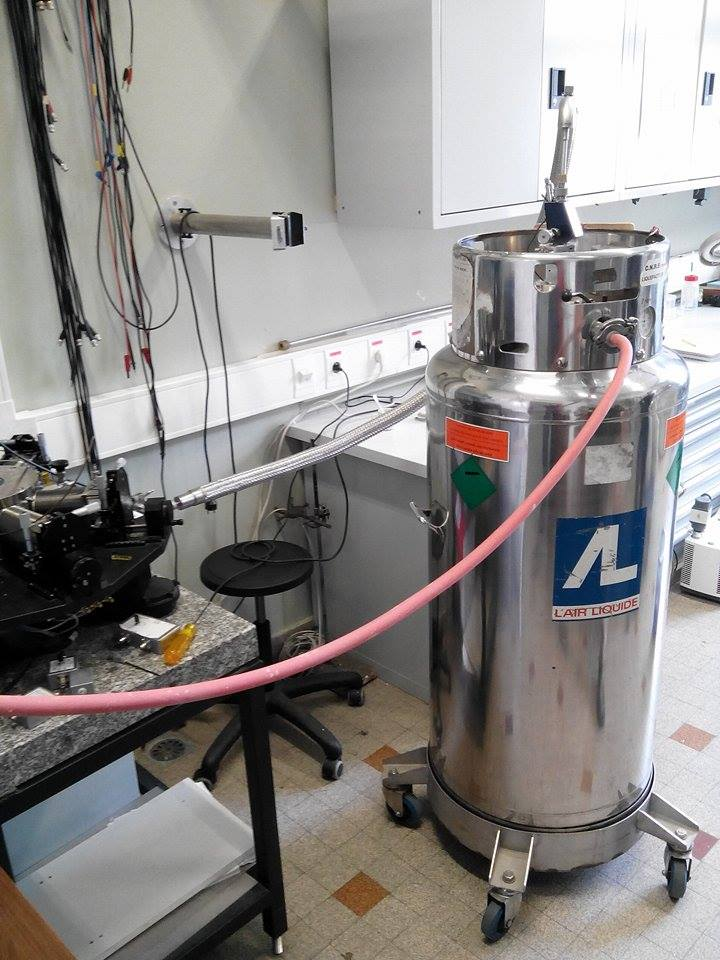
\includegraphics[width=150px]{Photos/Bouteille_Helium_Liquide.jpg}
        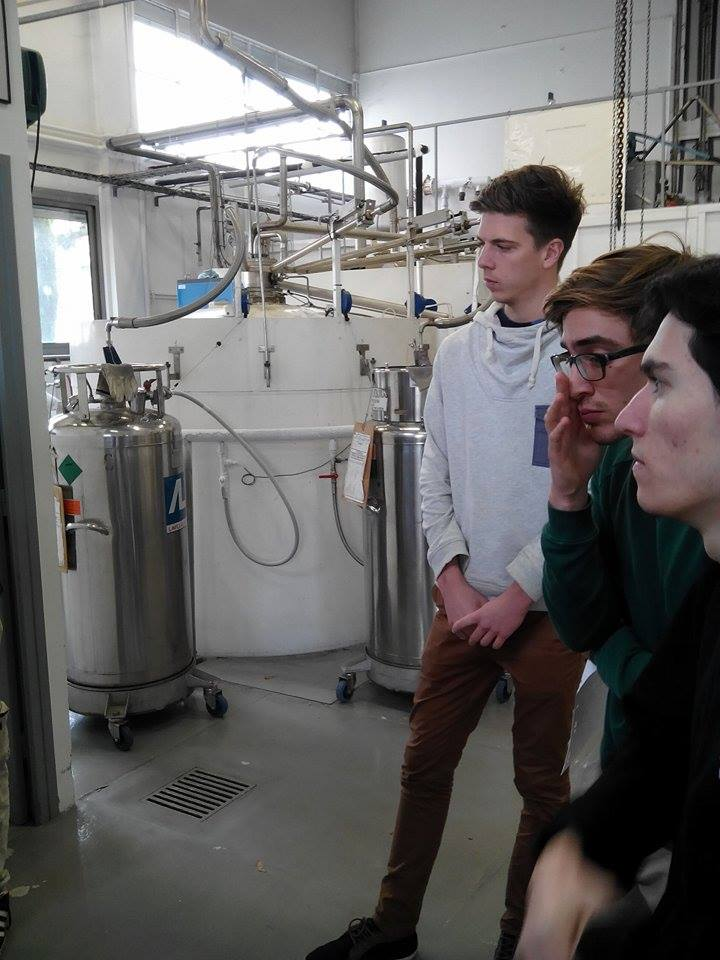
\includegraphics[width=150px]{Photos/Centre_Helium_Liquide.jpg}
        \caption{Une bouteille d'Hélium Liquide et le centre de liquéfaction.}
        \label{fig:}
    \end{center}
\end{figure}

\section{Les méthodes de mesure}
\subsection{La mesure de résistivité}
Afin de vérifier que nos pointes sont bien connectées et qu'il y a bien un nanofil entre elles, on utilise un ohmmètre spécialisé délivrant des micro-ampères. En effet la largeur de transport est de quelques atomes d'or et un courant classique de l'ordre du mA détruirait immédiatement nos échantillons.
Nous polarisons nos échantillons en tension, et cherchons donc à mesurer le courant traversant les échantillons.
On transforme le courant en une tension par l'intermédiaire d'un convertisseur courant-tension présentant différents facteurs, afin d'effectuer nos mesures. Lors de l'électromigration on utilise un facteur $10^3$ pour mesurer des uA.
Pour observer les diamants de Coulomb on mesure des faibles courant (nA),  on sélectionne le facteur $10^6$ sur le convertisseur. 

\begin{figure}[h]
    \begin{center}
        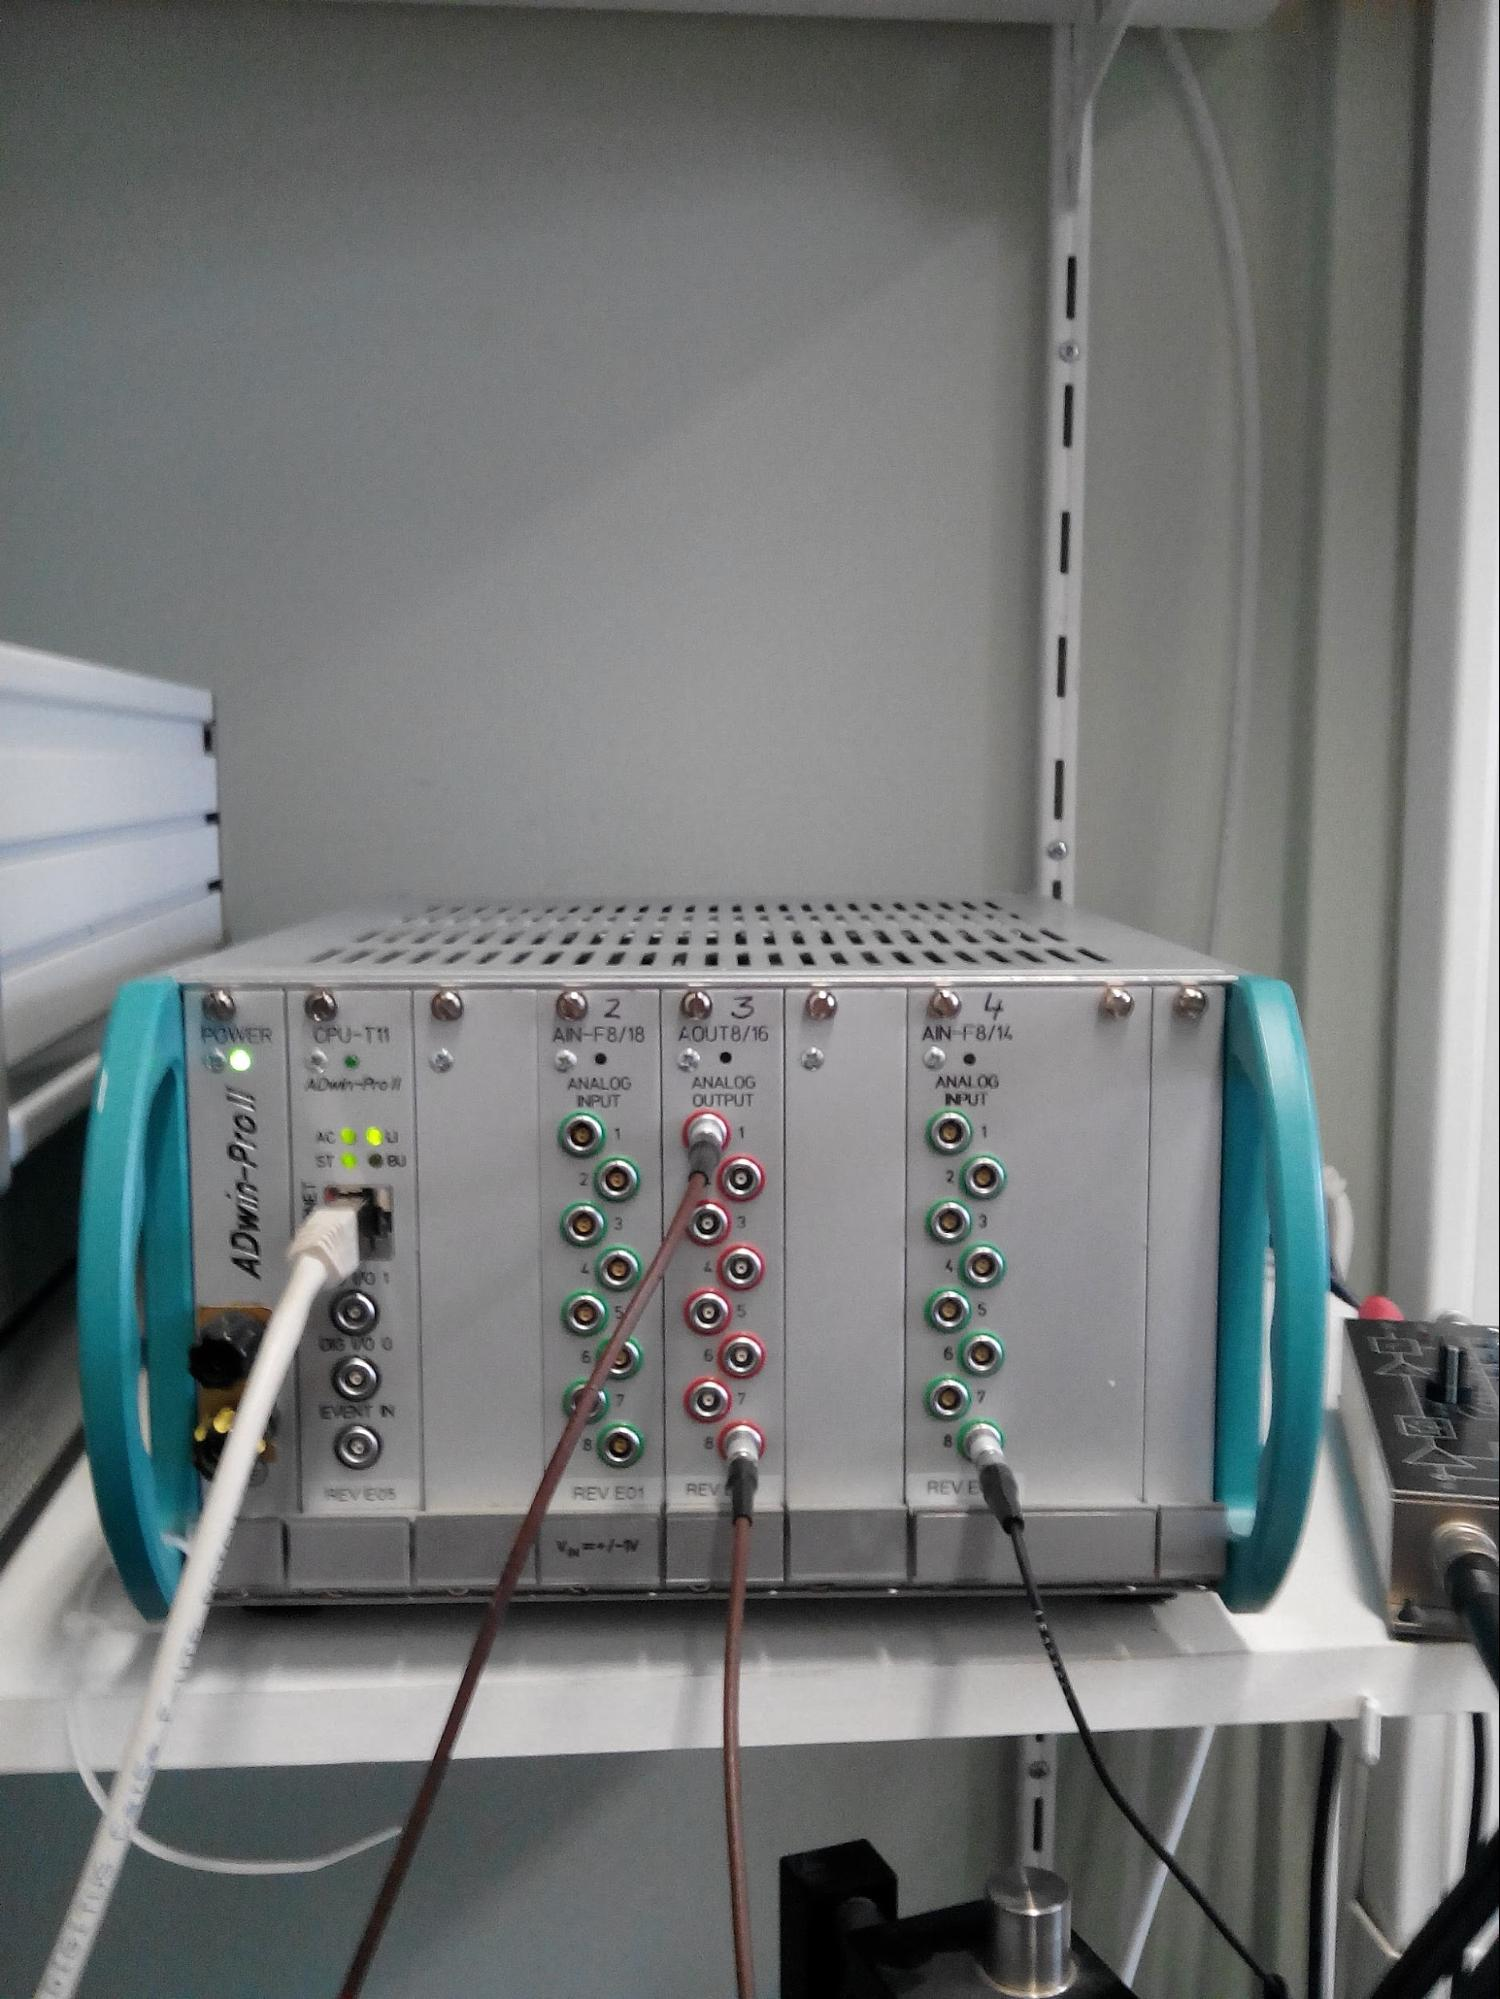
\includegraphics[trim=0mm 0mm 80px 600px, clip, width=200px]{Photos/Branchements_ADWin.jpg}
        \caption{Branchements de l'interface Adwin lors de l'électromigration, on peut voir sur la droite le convertisseur courant-tension}
        \label{fig:}
    \end{center}
\end{figure}


\subsection{Les précautions à prendre}
Lorsqu'on manipule de tels échantillons, il faut bien sûr prendre quelques précautions afin de ne pas les détériorer définitivement.
Dans le testeur sous pointes, les échantillons sont à l'abri des perturbations extérieures : la structure de l'appareil, et particulièrement le plateau sur lequel les échantillons sont posés, sont mis à la masse.
Le principal risque vient donc des pointes : Si on les fait bouger alors qu'une tension est appliquée, le risque de pics de tension est très élevé. Avant chaque mesure et déplacement des pointes, nous faisons donc attention à les mettre à la masse. Cela peut être répétitif, mais absolument indispensable. 

\section{L'électromigration}
L'électromigration consiste, comme nous l'avons expliqué précédemment, à appliquer à l'échantillon une tension suffisamment forte pour “détruire” le fil d'or et créer un nanogap.
ADWin nous permet d'avoir une mesure suffisamment rapide du courant et d'arrêter l'électromigration suffisamment rapidement pour ne pas risquer d'abîmer le nanogap créé.
Nous pouvions observer en temps réel les courbes de courant et de résistivité de l'échantillon. Pour un échantillon correct nous observions bien la rampe de tension appliquée puis le comportement classique d'électromigration, dont la chute par paliers du courant.
Pour un échantillon abîmé -- ce fut malheureusement le cas pour beaucoup, dû à un problème en salle blanche en amont --, nous pouvions observer une résistivité qui croit linéairement dès l'application de la tension.
\section{L'étude du blocage de Coulomb}
Après avoir effectué l'électromigration avec succès sur un échantillon, il nous fallait vérifier la présence d'une molécule de Fullerène dans le nanogap tout juste créé.  Pour cela, on mesure le courant Id en faisant varier la tension appliqué à la grille. Si aucun courant n'est observé, alors aucune molécule de Fullerène ne s'est logée à l'intérieur du nanogap. Si l'on observe des pics de courant pour certaines valeurs discrètes de Vg, c'est que l'on est en présence d'une boite quantique. Lorsque les conditions sont vérifiées par rapport aux équations établies dans la partie théorique, le courant peut passer ou non. On contrôle donc un courant  à partir d'une tension appliquée à une électrode de grille : on vient donc de réaliser un transistor à molécule unique.

On peut aussi observer le courant pour des valeurs variables de Vg et Vds. Le courant Id mesuré est représenté en 3ème dimension ou en couleurs. Nous pouvons alors observer la forme caractéristique des diamants de Coulomb, dont la frontière correspond aux pics de courant évoqués précédemment.

    
\chapter{Résultats obtenus}
\section{Électromigration}
\begin{figure}[h]
    \begin{center}
        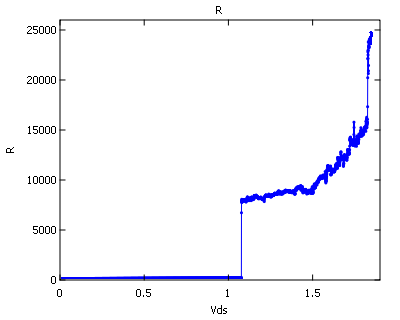
\includegraphics[width=150px]{Images/Image_Electromigration_1.png}
        \caption{La caractéristique R = f (V$_{ds}$)}
        \label{fig:}
    \end{center}
\end{figure}
On envoie un rampe de tension allant de 50mV à 2,5V avec une vitesse de 5mV/s.
L’énergie est dissipé par effet Joule et induit des vibrations du réseau cristallin. Après 1,2V  on commence à casser petit à petit la jonction jusqu’à créer le nanogap. Expérimentalement on observe Rmax=12,9kOhm pour un unique canal d’or et Rmax=25kOhm au moment de la formation du nanogap. On arrête donc l’électromigration lorsque l’on atteint R=25kOhm.
Grâce au système de mesure en temps réel on peut obtenir facilement la courbe R = f(Vds). Si l’électromigration est réussie on obtient une courbe du type de celle ci dessus, il est possible cependant que le nanofil soit déjà endommagé avant électromigration (résistance déjà de l’ordre de quelques kOhms). 

La mobilité des atomes est activée par la température. Localement (au niveau du nanogap) la température est de l’ordre de 400K lors de l’électromigration [11]. Cependant l’arrêt de l’électromigration en une microseconde, et les dimensions concernées très faibles empêchent pas une élévation globale de l’échantillon en température.
\section{Observation du blocage de Coulomb}
Pour savoir si une molécule de C60 est tombé dans le nanogap, On trace la caractéristique I(V) pour différentes valeurs de la tension de grille Vg. L’influence de la boite quantique produira différentes caractéristiques, au contraire les caractéristiques seront toutes confondues si le gap est vide.
 Notons bien qu’il faut toujours utiliser des rampes de tensions entre la connexion et la déconnexion pour ne pas casser les les fronts montants ou descendants en voyant des fronts d’une amplitude de 1V.
 \begin{figure}[h]
    \begin{center}
        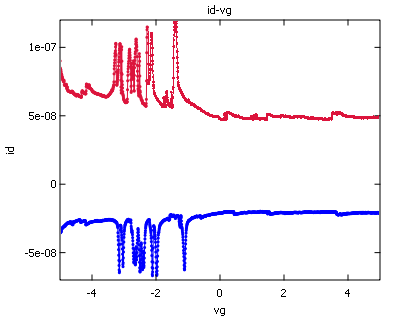
\includegraphics[width=150px]{Images/Image_Blocage_Coulomb_1.png}
        \caption{Id=f(Vg) on observe bien des pics de Coulomb (ici il pourrait s’agir d’un unique pic)}
        \label{fig:}
    \end{center}
\end{figure}
Sur la courbe Vds(Vg) on cherche à observer les diamants de Coulomb. Les différents pics mesurés doivent être également présents lorsqu’on envoie un tension drain-source négative, on est alors sur d’avoir non pas du bruit mais bien un pic lié au blocage de Coulomb.
Malheureusement nous n’avons pas pu mesurer des diamants de Coulomb exploitable, selon Franck Balestro 1 transistor sur 100 donne des résultats d’une bonne qualité.

\section{Quelques cas particuliers}
Après ces considérations générales étudions quelques cas particuliers, et plus précisément des observations obtenues lorsque des problèmes ont été rencontrés au cours de l’expérience.
 \begin{figure}[h]
    \begin{center}
        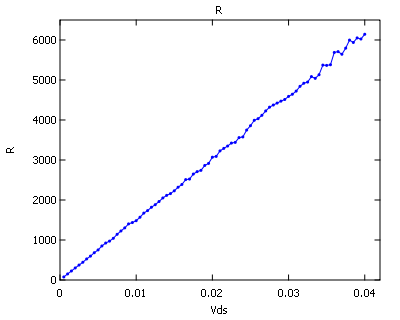
\includegraphics[width=150px]{Images/Nanofil_Emdommage.png}
        \caption{Nanofil endommagé avant électromigration}
        \label{fig:}
    \end{center}
\end{figure}

 \begin{figure}[h]
    \begin{center}
        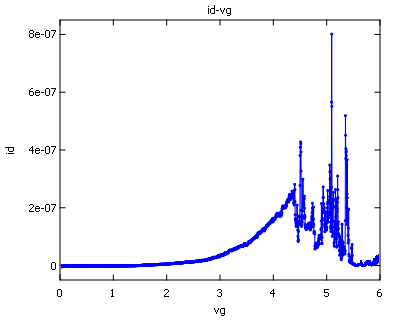
\includegraphics[width=150px]{Images/Grille_Endommagee}
        \caption{Grille endommagée}
        \label{fig:}
    \end{center}
\end{figure}

 \begin{figure}[h]
    \begin{center}
        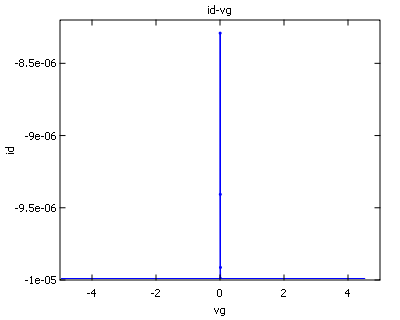
\includegraphics[width=150px]{Images/Grille_Detruite}
        \caption{Grille détruite (au delà de Vg=7V on détruit la grille)}
        \label{fig:}
    \end{center}
\end{figure}






\chapter{Aller plus loin ? Vers de nouvelles expériences…}
\section{Une expérience à 20mK}
Les éxpériences actuelles de l'équipe NanoSpin n'utilisent ni des molécules de Fullerène, ni un testeur sous pointes et n'ont pas lieu à 4,2K. De plus le convertisseur courant-tension n'est pas un modèle commercial mais a été fabriqué au CNRS pour permettre des mesures ultra bas bruit.

En effet la molécule de Fulerène n'ayant aucune propriété particulière elle a été rapidement remplacé par des molécules aux propriétés plus intéressantes, notamment les aimants moléculaires dont nous parlions en introduction. Par exemple TbPc2 dans le cas de l'équipe de nanospintronique et transport moléculaire.
Les contacts par pointes sont aussi remplacés par des micro-soudures qui possèdent plusieurs avantages sur le contact par pointes. Bien qu'une telle technique soit plus délicate et plus longue à mettre en place et ne permette de tester les transistors qu'en faible nombre, elle a comme intérêts majeurs de réduire le bruit, et permettre un contact parfait sur des durées très longues (certaines expériences sont en cours depuis plus d'un an)

\begin{figure}[h]
    \begin{center}
        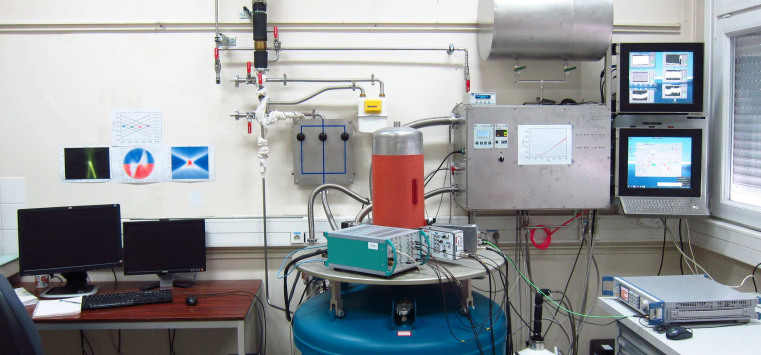
\includegraphics[width=150px]{Images/5_Refrigerateur_Dillution.jpg}
        \caption{Photographie du réfrigérateur à dilution et de l'ensemble du banc de mesure}
    \end{center}
\end{figure}

Pour finir, l'expérience actuelle se déroule actuellement à des températures de 30mK dans un réfrigérateurs à dilution, la température de électronique étant elle de l'ordre de 80mK \cite{10}. Le principe du réfrigérateur à dilution est comparable à celui d'un réfrigérateur classique, des détentes de Joule-Thomsom successives pour refroidir l'hélium à de très basses températures. Le réfrigérateur étant constitué de différents étages dont les températures vont en diminuant pour limiter les pertes. Il faut cependant attendre plusieurs heures pour qu'une température de 30mK soit atteinte.
\section{Vers l'information quantique ?}

L'information quantique se définit comme “la théorie de l'utilisation des spécificités de la physique quantique pour le traitement et la transmission de l'information” \cite{18}. L'utilisation de telles propriétés permettraient d'obtenir des supports et du traitement de l'information bien plus efficaces qu'actuellement.

Bien que l'ordinateur quantique ne soit qu'un but à long (voire très long) terme, la réalisation de transistors de spin à base d'aimants moléculaires est possible. La manipulation et la lecture de spins nucléaires uniques i.e. l'utilisation des propriétés quantiques des aimants moléculaires est permise grâce à des dispositifs comparables à ceux que nous avons utilisés. Ces aimants moléculaires utilisés comme qubits sont ainsi d'excellents candidats pour le stockage de l'information quantique, ils respectent en effet les 5 critères de Divincenzo pour le traitement de l'information quantique.[12] Les critères de Divincenzo définissant quels qubits sont exploitables et assez stables pour effectuer des calculs utiles.


\chapter*{Conclusion}
Durant ce projet de recherche, nous avons vu comment réaliser un transistor de type SET (Single Electron Transistor) à l'aide d'une molécule de fullerène. Cette idée de créer des transistors à partir de molécules organiques est apparu dans les années 1970. Ce n'est seulement que dans les années 1990 que nous verrons l'apparition des premiers transistors à molécule unique. \medskip 

La réalisation d'un tel transistor se fait évidement en plusieurs étapes:

La première consiste à créer des nanofils d'or sur une plaque de Al$_2$0$_3$ où nous déposerons ensuite les molécules de fullerène. Ce dépôt se fait avant l'électromigration car cela augmente les chances qu'une molécule se loge dans un nanogap créée par l'électromigration.

Vient ensuite l'étape de l'électromigration. Elle consiste à appliquer un courant tel que les électrons emportent les atomes d'or qui constituent les nanofils grâce à leur énergie cinétique. En créant ces nanogaps, une molécule de fullerène peut se loger à l'intérieur et ainsi créer notre boite quantique. 

Le dépôt de fullerène et la création de nanogaps peuvent se suivre en direct grâce au testeur sous pointes et le logiciel ADWin. Par exemple, il permet de suivre en direct l'augmentation de la résistance du nanogap durant l'électromigration, de savoir s'il reste des canaux par où passent les électrons et donc de savoir si le nanogap a été formé (on trouvera une résistance R$_\text{max}$=25k$\Omega$). La caractéristique I(Vg) permettra quant à elle de savoir si oui ou non une molécule de fullerène est dans le nanogap. Ces instruments permettent donc à la fois la création des SET et la mesure de leurs caractéristiques.

Cette technologie a vu le jour dans les années 90. Mais la difficulté d'utilisation de ce type de transistor, notamment parce qu'il faut se placer à de très basse température (4,2K). Les chercheurs actuels ont remplacé la molécule de fullerène par de nouvelles molécules, le TbPc$_2$ par exemple. Cette molécule est très utilisée car elle permet la lecture et la manipulation d'un spin nucléaire. Mais la recherche ne s'arrête pas là: effectivement, l'équipe de Franck Balestro travaille actuellement avec plusieurs équipes de chimistes à travers le monde dans le but de trouver de nouvelles molécules intéressantes pour avancer dans le domaine de la spintronique.

\section*{Avis sur le projet de recherche}

Cet exercice de projet de recherche a été très enrichissant pour toute personne s'intéressant au monde de la recherche. Il nous a permis dans un premier temps de nous intéresser à un sujet très actuel sur lequel des chercheurs de Grenoble et du monde entier s'intéressent en ce moment. De plus, ce sujet était en relation direct avec le cours de Nanophysique dispensé en 2e année à Phelma en PNS. Pouvoir mettre en pratique des phénomènes jusque là seulement étudié en théories est évidement très grisant.

L'exercice du 1er semestre nous a permis de voir comment débuter et menée une bibliographie sur un sujet que nous maîtrisions pas dans sa globalité. Il nous a fallu une certaine dose d'indépendance et de travail personnel pour comprendre les tenants et les aboutissants de ce sujet
L'expérience menée au 2e semestre à durée une journée et il nous est apparu clair qu'il faut s'armer de patience si l'on veut trouver des résultats fiables et exploitables. Elle nous a aussi permis de suivre le quotidien d'un chercheur, bien que l'expérience menée n'était quant à elle pas tout à fait d'actualité.


\bibliographystyle{unsrt}
\bibliography{bibliographie}
\end{document}
